\section{Аналитическая часть}	
	\subsection{Обзор существующих аналогов}
	В настоящий момент существует несколько сервисов, выполняющих похожие задачи.
	
	\subsubsection{Геопортал охотничьего хозяйства России}
	Этот портал предоставляет удобный сервис для наилучшего ориентирования пользователей среди разнообразных охотничьих хозяйств. Он включает в себя набор интерактивных карт субъектов Российской Федерации с возможностью перехода по клику на информационную страницу, соответствующую выбранному элементу. \cite{maps} \\
	
	Однако набор действий на сайте очень ограничен. Так, ссылки, указывающие на возможность приобретения путёвки на охоту, перенаправляют пользователя либо на инструкцию, в которой указано, какое учреждение нужно очно посетить для оформления соответствующих документов, либо на сайт с уже устаревшей информацией. И лишь некоторые субъекты перенаправляют на сайт Госуслуг для подачи заявки онлайн. Личного кабинета у пользователя на этом портале нет. \\
	
	\subsubsection{Портал государственных и муниципальных услуг}
	Сервис поддерживает подачу заявок онлайн, для этого необходимо заполнить формы и подгрузить необходимые документы. Но также обязательным условием является посещение МФЦ. Все оформленные путёвки появляются в специально отведённом разделе в личном кабинете.\\
	
	Основным неудобством в работе данных сервисов является отсутствие возможности оформления документов на охоту удалённо, в любом случае, требуется посещение специального учреждения. Также ввиду ограниченного функционала личный кабинет либо отсутствует, либо предоставляет только общую информацию, за детальным разъяснением приходится обращаться в сторонние сервисы. Поэтому в качестве одной из задач данной работы ставится выполнение указанных требований.
	
	\subsection{Формализация задачи}
	В ходе выполнения курсовой работы должно быть спроектировано и реализовано Web-приложение, предоставляющее интерфейс для работы с данными о членах организации, путёвках, прайс-листах для различных категорий пользователей (таких как, администратор, егерь, охотник). Для каждого участника должен быть определён свой набор прав и разрешённых действий.\\
	
	Кроме того, необходимо обеспечить возможность регистрации с дальнейшим подтверждением со стороны администратора. В случае положительного ответа пользователю предоставляется функционал в соответствии с его категорией.
	
	\subsection{Формализация ролей}
	Было выделено три категории пользователей.\\
	
	\textbf{Охотник} \\
		Может выполнять следующие действия.
		\begin{itemize}
			\item Просматривать:
			\begin{itemize}
				\item личную информацию;
				\item контакты всех егерей занесённых в базу данных;
				\item свои одобренные путёвки и заявки на их покупку;
				\item прайс-лист по всем хозяйствам и секторам с возможностью поиска необходимого субъекта.
			\end{itemize}
			\item Отправлять:
			\begin{itemize} 
			 	\item заявки на путёвки с указанием места охоты и количества животных.
			\end{itemize}
		 	\item Отзывать:
		 	\begin{itemize}
		 		\item созданную ранее заявку.
		 	\end{itemize}
		\end{itemize}
	
		\textbf{Егерь} \\
		Ему предоставляются следующие возможности.
		\begin{itemize}
			\item Просматривать:
			\begin{itemize}
				\item личную информацию;
				\item общую информацию о всех охотниках с возможностью поиска по ФИО и номеру охотничьего билета;
				\item контакты всех егерей занесённых в базу данных;
				\item прайс-лист закреплённого за ним сектора с возможностью поиска необходимого животного;
				\item заявки на охоту, а также одобренные путёвки в его сектор.
			\end{itemize}
			\item Отклонить или принять:
			\begin{itemize} 
				\item заявку на путёвку в его сектор.
			\end{itemize}
			\item Оформить:
			\begin{itemize} 
				\item новую путёвку в закреплённый за ним сектор с указанием номера билета охотника и позиции из доступного прайс-листа.
			\end{itemize}
			\item Закрыть:
			\begin{itemize}
				\item уже одобренную путёвку.
			\end{itemize}
			
		\end{itemize}
		
		\textbf{Администратор}\\
		Для него определён соответствующий набор действий.
		\begin{itemize}
			\item Просматривать:
			\begin{itemize}
				\item личную информацию;
				\item информацию о всех охотниках, занесённых в базу данных, с возможностью поиска по ФИО и номеру билета;
				\item информацию о всех егерях, занесённых в базу данных, с возможностью поиска по ФИО и субъекту;
				\item информацию о всех администраторах, занесённых в базу данных, с возможностью поиска по ФИО;
				\item заявки на охоту во всех возможных хозяйствах и секторах;
				\item заявки на регистрацию в качестве охотника, егеря, администратора;
				\item выданные путёвки во всех возможных хозяйствах и секторах.
			\end{itemize}
			\item Отклонить или принять:
			\begin{itemize} 
				\item заявку на охоту в любой субъект;
				\item заявку на регистрацию в качестве охотника, егеря, администратора.
			\end{itemize}
			\item Оформить:
			\begin{itemize} 
				\item новую путёвку с указанием названия хозяйства, номера сектора, номера билета охотника и позиции из доступного прайс-листа.
			\end{itemize} 
			\item Закрыть:
			\begin{itemize}
				\item уже одобренную путёвку из любого субъекта.
			\end{itemize}
			\item Удалить аккаунт:
			\begin{itemize} 
				\item охотника;
				\item егеря;
				\item администратора (кроме себя самого).
			\end{itemize}
		\end{itemize}
	
	\subsection{Формализация данных}
	На рисунке \ref{fig1:image} приведена ER-диаграмма схемы сущностей.
	
	\begin{figure}[ph!]
		\centering
		\begin{center}
			{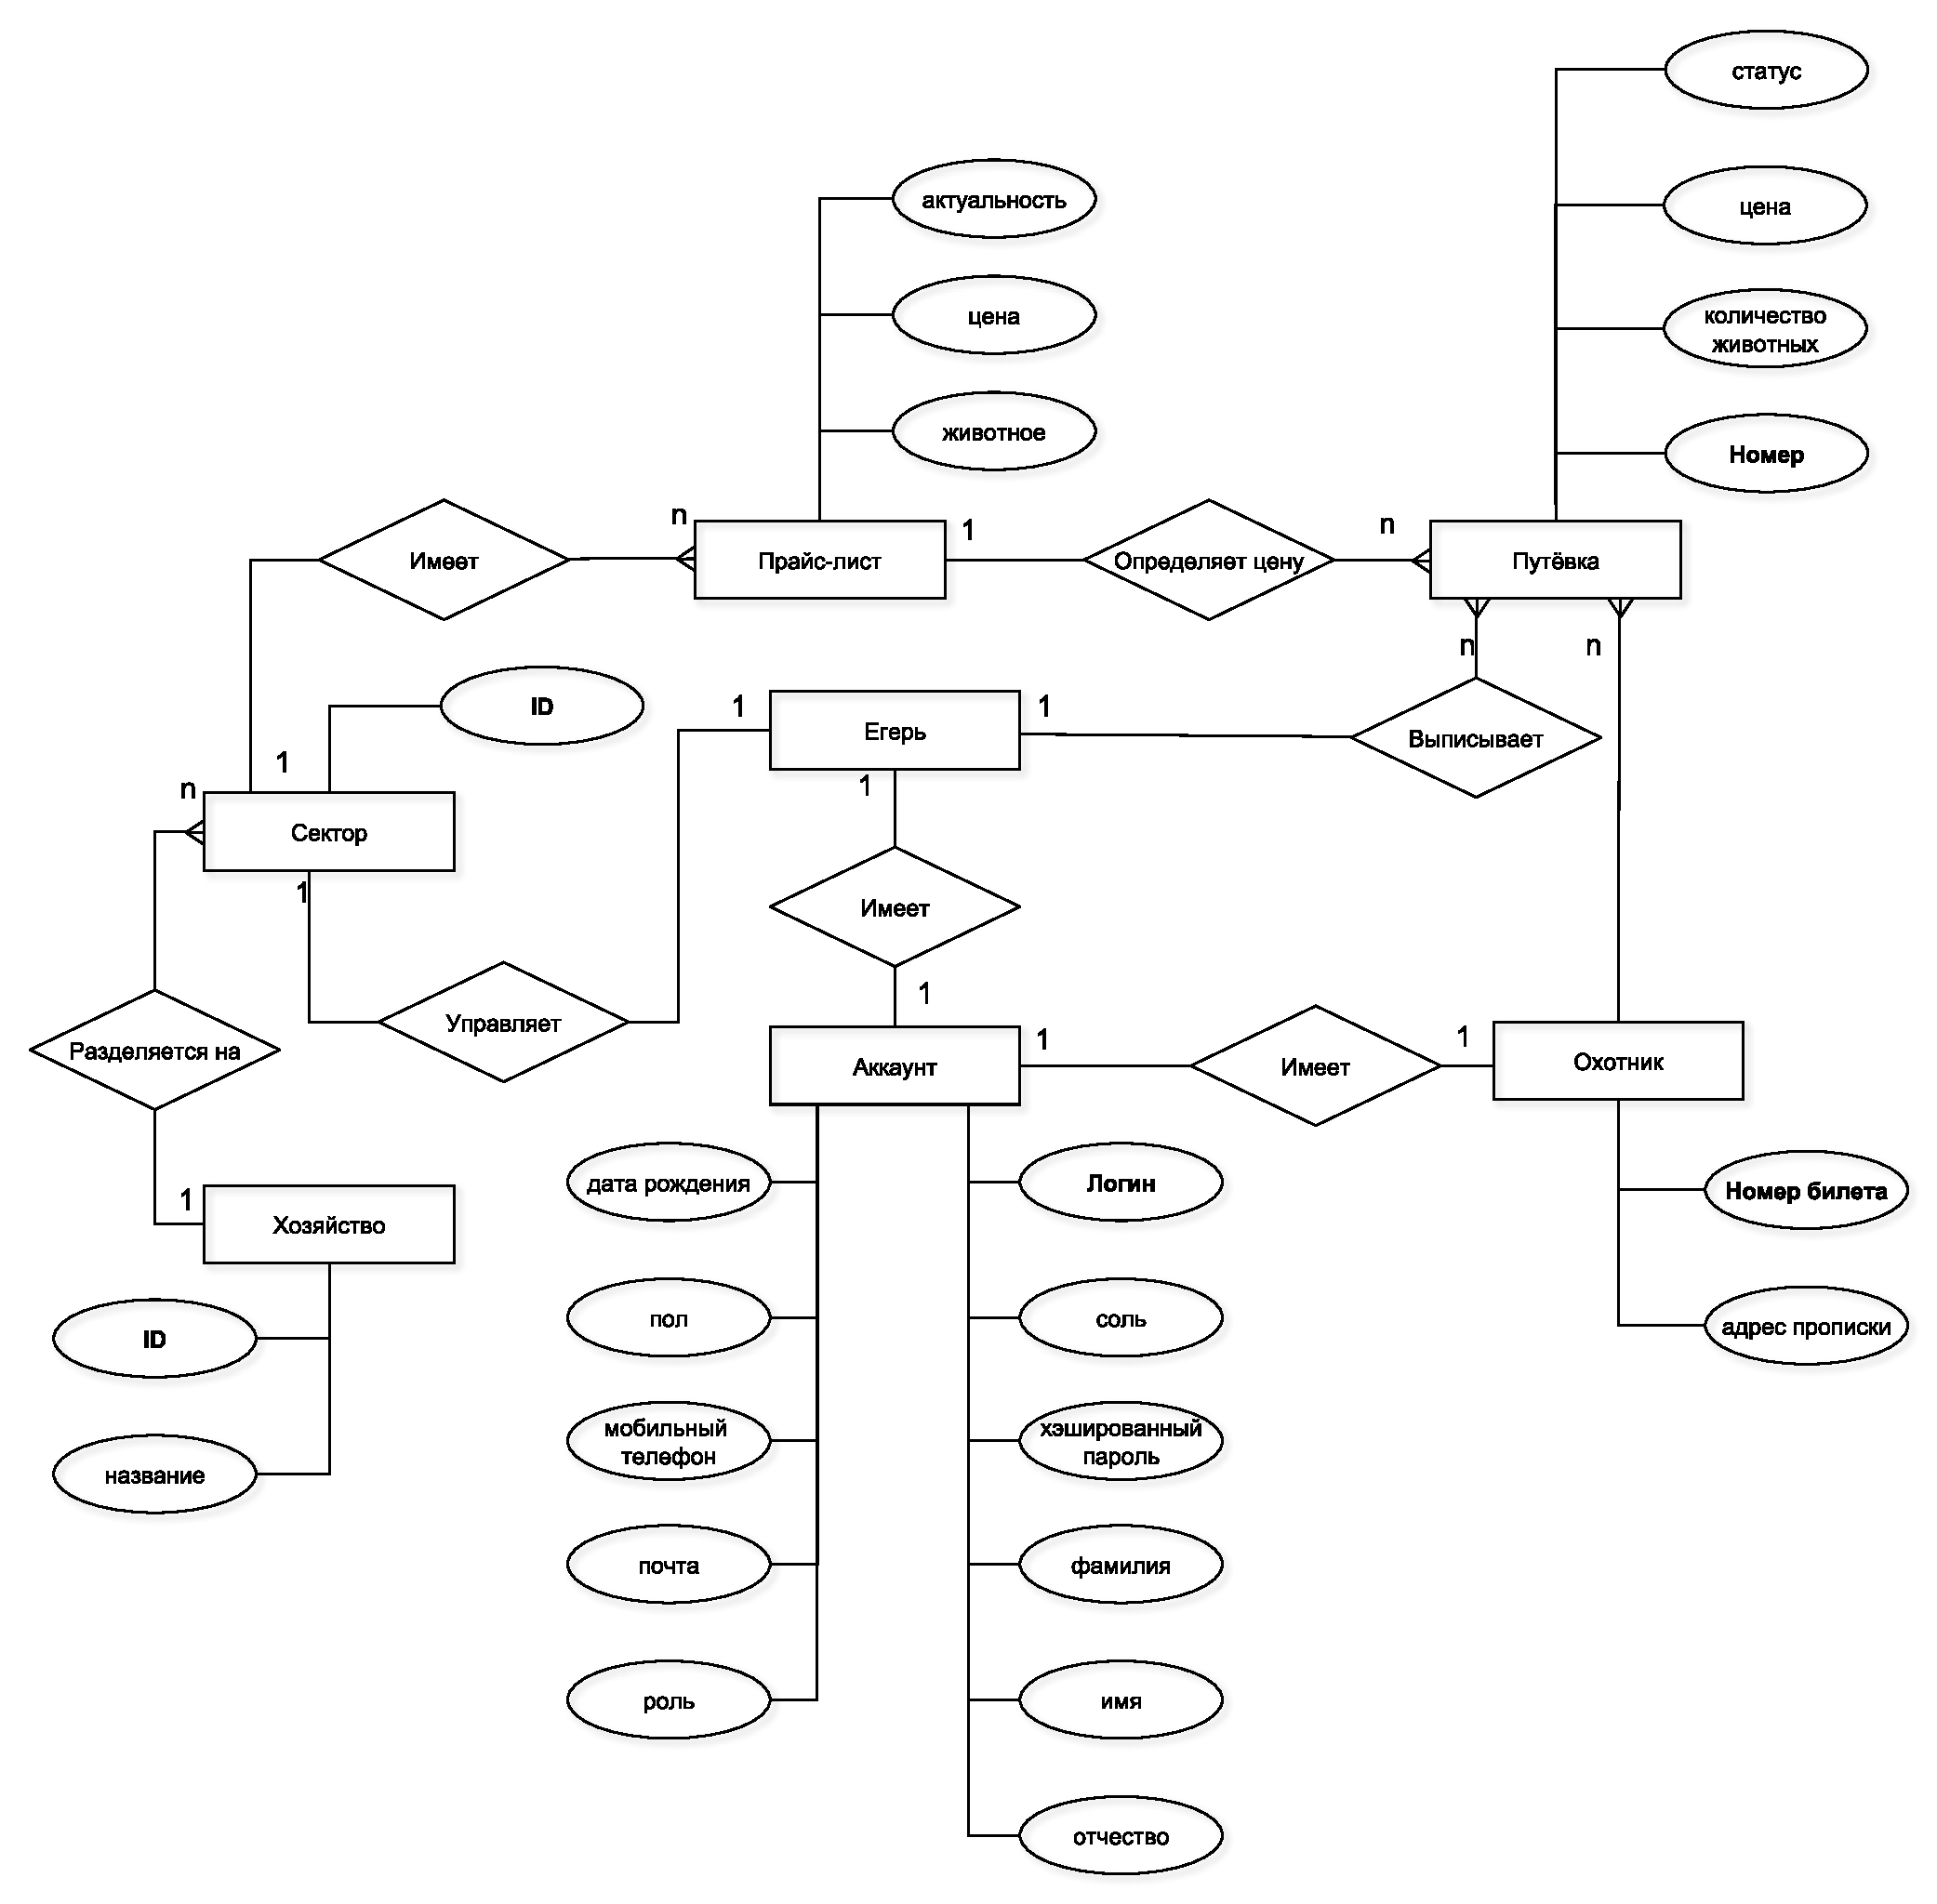
\includegraphics[scale=0.45]{schemes/er.pdf}}
			\caption{ER-диаграмма сущностей}
			\label{fig1:image}
		\end{center}
	\end{figure}

	\newpage

	\subsection{Базы данных}
	\subsubsection{Определение базы данных}
	\textbf{База данных (БД)} -  это самодокументированное собрание интегрированных записей.\\
	\textbf{Самодокументированная} - хранятся метаданные (данные о данных).\\
	\textbf{Интегрированные записи} – файлы данных.
	
	\subsubsection{Требования к БД}
	\begin{enumerate}
		\item[1)] Неизбыточность \\
		Не хранится лишняя информация.
		\item[2)] Эффективность доступа \\
		Малое время отклика на запрос.
		\item[3)] Совместное использование
		\item[4)] Безопасность
		\item[5)] Восстановление после сбоя
		\item[6)] Целостность \\
		Если есть ссылка на какой-то объект, то он должен быть. Нельзя ссылаться на несуществующие объекты.
		\item[7)] Независимость от сторонних приложений
	\end{enumerate}

	\subsubsection{Модели данных}
	\textbf{Модель данных} - это абстрактное, самодостаточное, логическое определение объектов, операторов и прочих элементов, в совокупности составляющих абстрактную машину доступа к данным, с которой взаимодействует пользователь. Эти объекты позволяют моделировать структуру данных, а операторы — поведение данных. \cite{db} \\
	
	Выделяют три основные модели данных.
	\begin{enumerate}
		\item[1)] Иерархическая \\
		Подразумевается, что элементы организованы в структуры, связанные между собой иерархическими или древовидными связями. Родитель может иметь несколько потомков. Но у потомка может быть только один предок.
		\item[2)] Сетевая \\
		У родителя также может быть несколько потомков, а у дочернего элемента — несколько предков.
		\item[3)] Реляционная \\
		Главное отличие состоит в том, что информация хранится в виде таблиц (отношений), состоящих из нескольких записей (кортежей), обладающих одним и тем же набором атрибутов, или полей. Используются чаще, чем две другие модели.
	\end{enumerate}

	Реляционная модель данных наиболее подходит для решения поставленной задачи, поскольку она более гибкая и удобна в использовании.
	
	\subsubsection{Система управления базами данных (СУБД)}
	\textbf{Система управления базами данных (СУБД)} - приложение, позволяющее создать базу данных и манипулировать данными (вставлять, обновлять, удалять и выбирать).\\
	Основные компоненты СУБД. \cite{db_systems}
	\begin{itemize}
		\item Ядро \\
		Отвечает за управление данными во внешней и оперативной памяти и журнализацию.
		\item Процессор языка БД\\
		Используется для оптимизации запросов на извлечение и изменение данных.
		\item Подсистема поддержки времени исполнения\\
		Интерпретирует программы манипуляции данными, создающие пользовательский интерфейс с СУБД.
		\item Сервисные программы\\
		Отвечают за обеспечение дополнительных возможностей.
	\end{itemize}

	\subsection*{Вывод}
	Был проведён обзор существующих решений, на основе анализа предоставляемых ими возможностей была формализована задача курсового проекта, также были определены категории пользователей и соответствующие им действия. Кроме того, приведены некоторые теоретические сведения, необходимые для дальнейшей работы.
	
	